\documentclass[xcolor=x11names,compress]{beamer}

%\newcommand*{\upbullet}{\includegraphics[width=1em]{QC8_8.3_psi.pdf}}
%\setbeamertemplate{itemize item}{\upbullet}

%% General document %%%%%%%%%%%%%%%%%%%%%%%%%%%%%%%%%%
\usepackage{graphicx}
\usepackage{tikz}
\usetikzlibrary{decorations.fractals}
\usetikzlibrary{arrows,shapes}
\usetikzlibrary{shapes.geometric}
\usetikzlibrary{shadows}
\usetikzlibrary{snakes}
\usetikzlibrary{decorations.text}
\usepackage{fancybox}
\usepackage{amsmath}
\usepackage{graphics}
\usepackage[latin1]{inputenc}
\usefonttheme{professionalfonts}
\usepackage{times}
\usepackage{verbatim}
\usepackage{ragged2e}
\usepackage[justification=centering]{caption}
\usepackage{fancybox}
\usepackage{CJK}
\usepackage{media9}

%% Beamer Layout %%%%%%%%%%%%%%%%%%%%%%%%%%%%%%%%%%

\useoutertheme[subsection=false, shadow]{miniframes}
\useinnertheme{default}
\usefonttheme{serif}
\usepackage{palatino}

\setbeamercovered{transparent}  	%<<<<<----------------- This sets transparent itemized lists.
%\usefonttheme[onlymath]{serif}   	%<<<<<----------------- Sets the font only for formulas.

\setbeamerfont{title like}{shape=\scshape}
\setbeamerfont{frametitle}{shape=\scshape}

\setbeamercolor*{lower separation line head}{bg=DeepSkyBlue4} 
\setbeamercolor*{normal text}{fg=black,bg=white} 
\setbeamercolor*{alerted text}{fg=red} 
\setbeamercolor*{example text}{fg=black} 
\setbeamercolor*{structure}{fg=black} 
 
\setbeamercolor*{palette tertiary}{fg=black,bg=black!10} 
\setbeamercolor*{palette quaternary}{fg=black,bg=black!10} 

\renewcommand{\(}{\begin{columns}}
\renewcommand{\)}{\end{columns}}
\newcommand{\<}[1]{\begin{column}{#1}}
\renewcommand{\>}{\end{column}}
\setbeamertemplate{navigation symbols}{}

%\setbeamertemplate{footline}[page number]
\setbeamertemplate{footline}
{
  \leavevmode%
  \hbox{%
  \begin{beamercolorbox}[wd=.28\paperwidth,ht=2.25ex,dp=1ex,center]{author in head/foot}%
    \usebeamerfont{author in head/foot}Joseph M. Fedrow  \end{beamercolorbox}%
  \begin{beamercolorbox}[wd=.44\paperwidth,ht=2.25ex,dp=1ex,center]{title in head/foot}%
    \usebeamerfont{title in head/foot}Git and LaTeX for Your Scientific Workflow \end{beamercolorbox}%
  \begin{beamercolorbox}[wd=.28\paperwidth,ht=2.25ex,dp=1ex,right]{date in head/foot}%
    \usebeamerfont{date in head/foot}\insertshortdate{}\hspace*{2em}
    \insertframenumber{} / \inserttotalframenumber\hspace*{2ex} 
  \end{beamercolorbox}}%
  \vskip0pt%
}


%%%%%%%%%%%%%%%%%%%%%%%%%%%%%%%%%%%%%%%%%%%%%%%%%%%%%%
%
%
\begin{document} 

\section{\scshape Introduction}
\subsection{Introduction}

\begin{frame}
\vspace{-0.5cm}
\title{
Git Your \LaTeX\,On!
}\author{
	Joseph M. Fedrow\\
	\vspace{0.5cm}
	\begin{tikzpicture}[decoration=Koch snowflake]
		\draw[DeepSkyBlue4] decorate{ decorate{ decorate{ (0,0) -- (3,0) }}};
	\end{tikzpicture}
	\vspace{-0.8cm}
}

\date{
	\today
	}
	
	\titlepage
	`
	\vspace{-0.5cm}
	
	
	
	 \centerline{
\includegraphics[scale=0.3]{asu-logo-E9CC4BDF34-seeklogo.com} \hspace{1.115cm}  
\includegraphics[scale=0.18]{asu-logo-DA1C895AD3-seeklogo.com}  \hfill{} 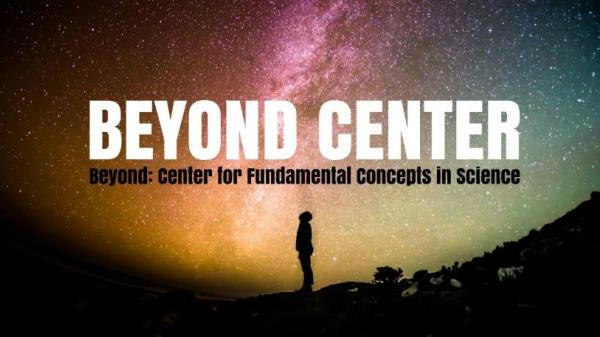
\includegraphics[scale=0.19]{Beyond Center Logo (New)}}

\end{frame}

\frame{
\frametitle{What are Git and LaTeX?}


\centerline{
\includegraphics[scale=0.2]{1}} 

\vfill

\centerline{Version control and Typesetting}

}

\frame{
\frametitle{How Can They Help You?}

\centerline{Version Control}

\vfill

\centerline{The practice of tracking and managing changes to source code over time}
\vfill

\centerline{Really shines when working in teams on collaborative projects.}

\vfill

\centerline{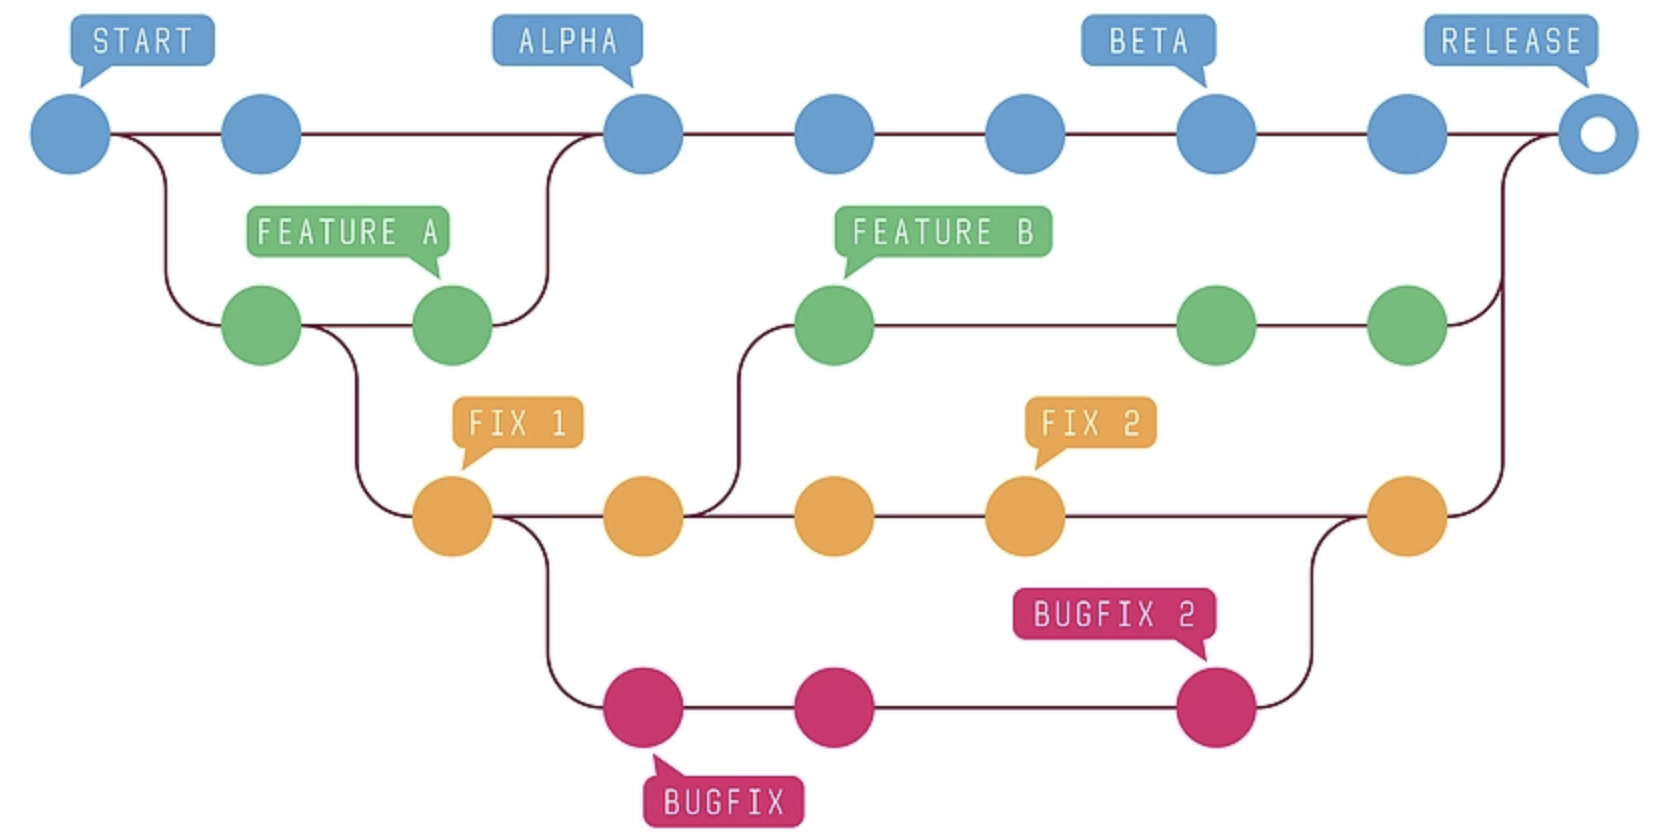
\includegraphics[scale=0.25]{3}} 



}

\frame{
\frametitle{How Can They Help You?}

\centerline{Typesetting}
\vfill

\centerline{Helps make your documents looks professional.}
\vfill
\centerline{Really shines when working with equations and tables.}
\vfill
\centerline{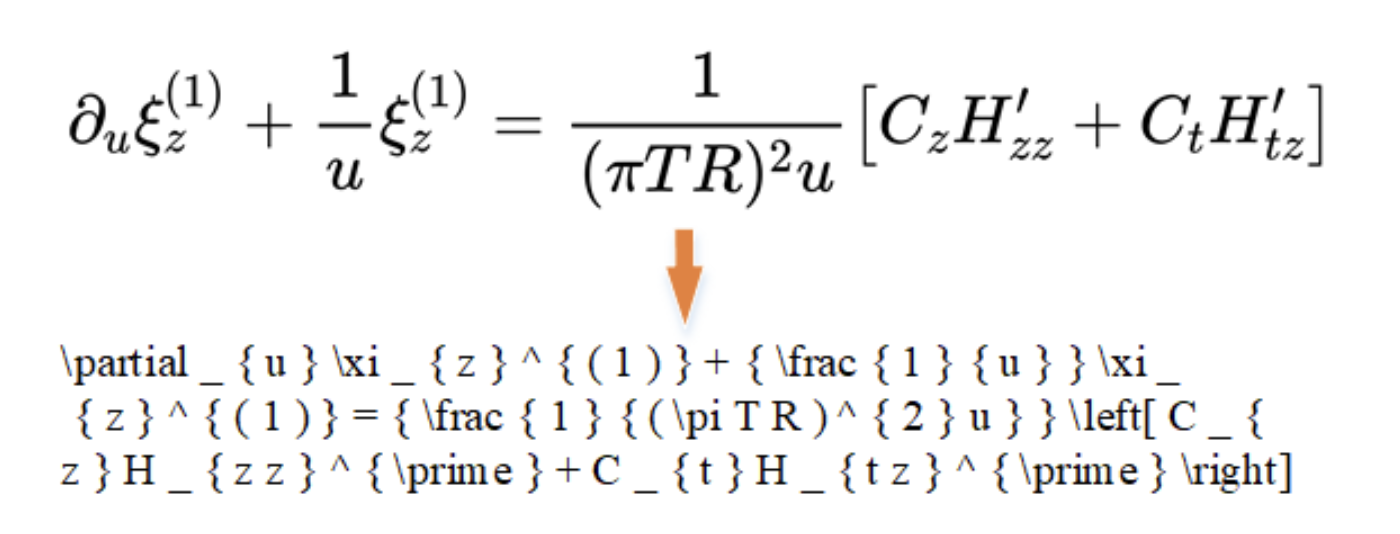
\includegraphics[scale=0.42]{4}} 

}


\section{\scshape Git}
\subsection{Git}

\frame{
\frametitle{The Philosophy of Git}

\centerline{Git is an open source \textit{Distributed} Version Control System (DVCS)}

\vfill

\centerline{Every clone is really a full backup of all the data.}

\vfill

\centerline{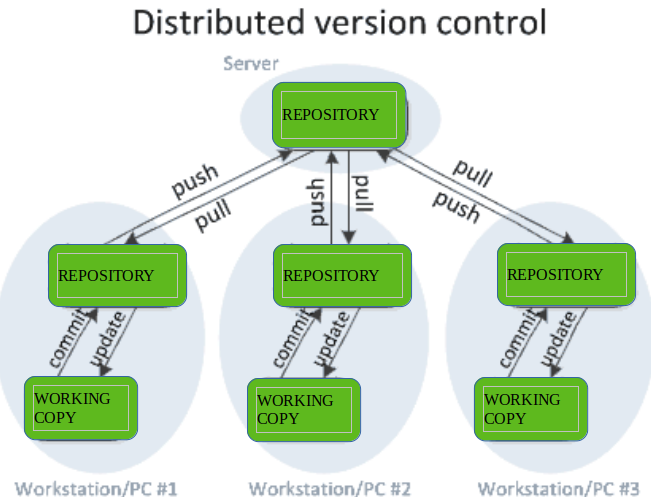
\includegraphics[scale=0.3]{8}}

}

\frame{
\frametitle{The Philosophy of Git}

\centerline{Nearly Everything is Local}
\vfill

\centerline{Snapshots of Data}
\vfill



\centerline{Git has Integrity}

\vfill

\centerline{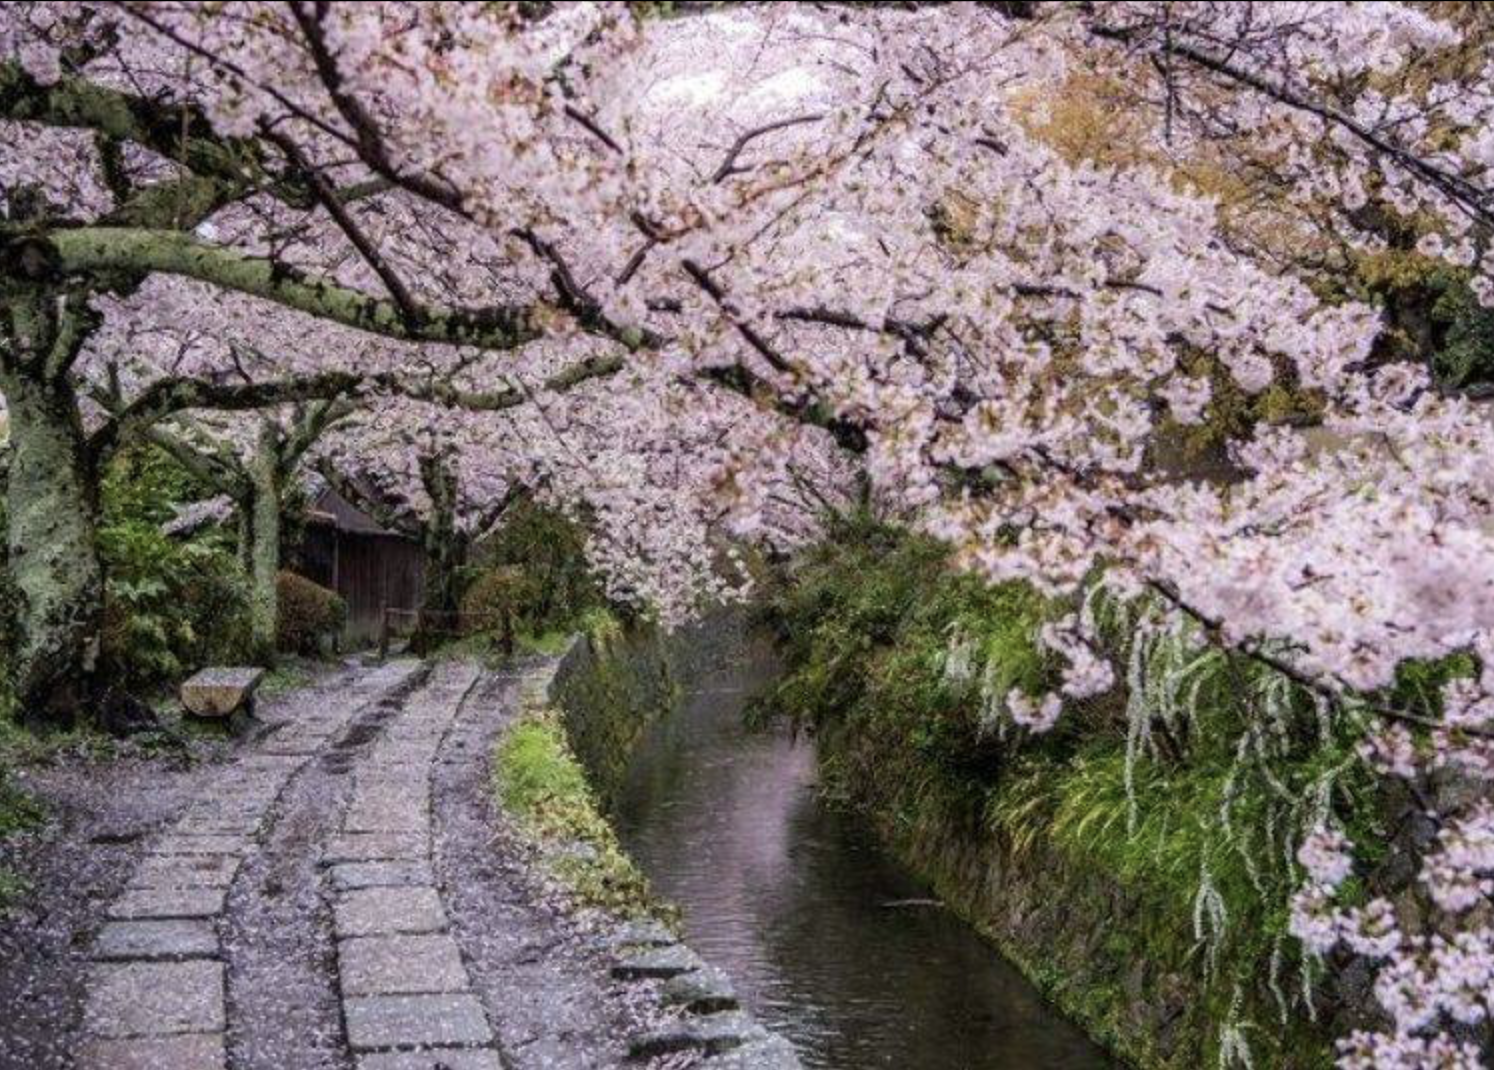
\includegraphics[scale=0.3]{17}}

}

\frame{
\frametitle{Bonus Question 1!}

\centerline{What does Git stand for?}

}

\frame{
\frametitle{Bonus Question 1!}

\centerline{What does Git stand for?}

\vfill

\centerline{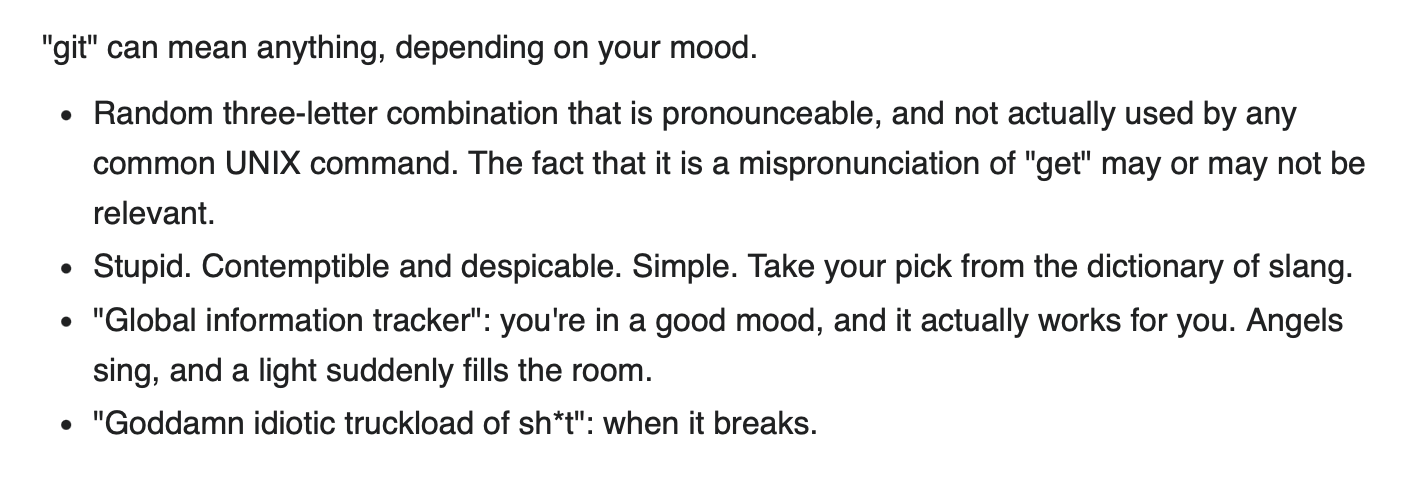
\includegraphics[scale=0.45]{12}}

}

\frame{
\frametitle{Bonus Question 1!}

\centerline{What does Git stand for?}
\vfill

\centerline{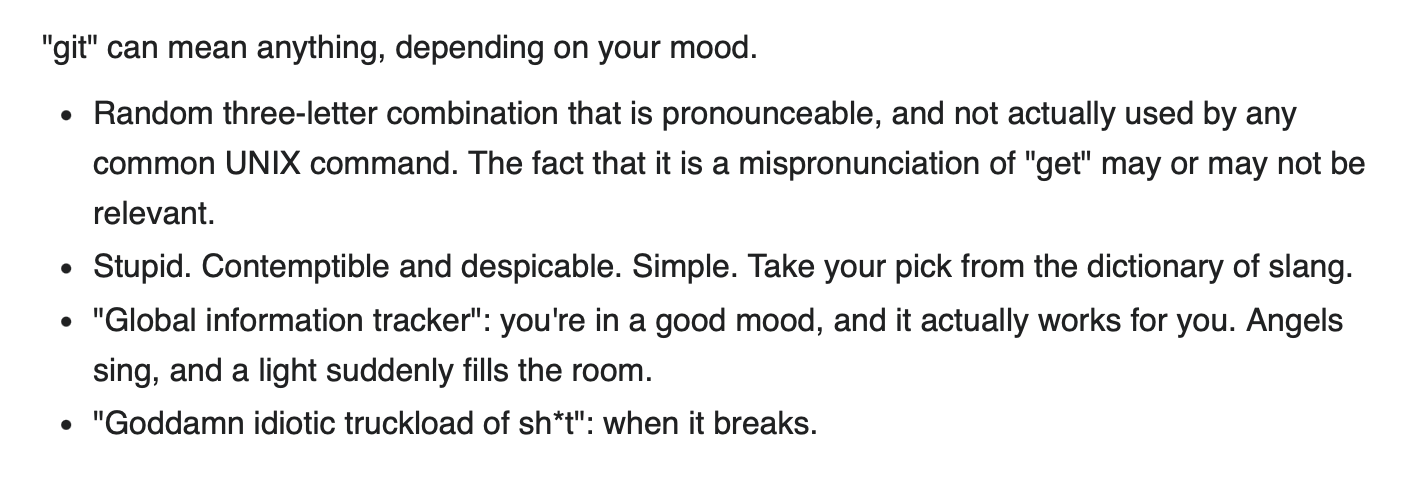
\includegraphics[scale=0.45]{12}}
\vfill

\centerline{
\includegraphics[scale=0.28]{11}}
\vfill
\centerline{Linus Torvalds, creator of Linux and Git}

}

\frame{
\frametitle{Git is not Github!}

\centerline{Git is a piece of software. GitHub is an online SaaS service.}

\centerline{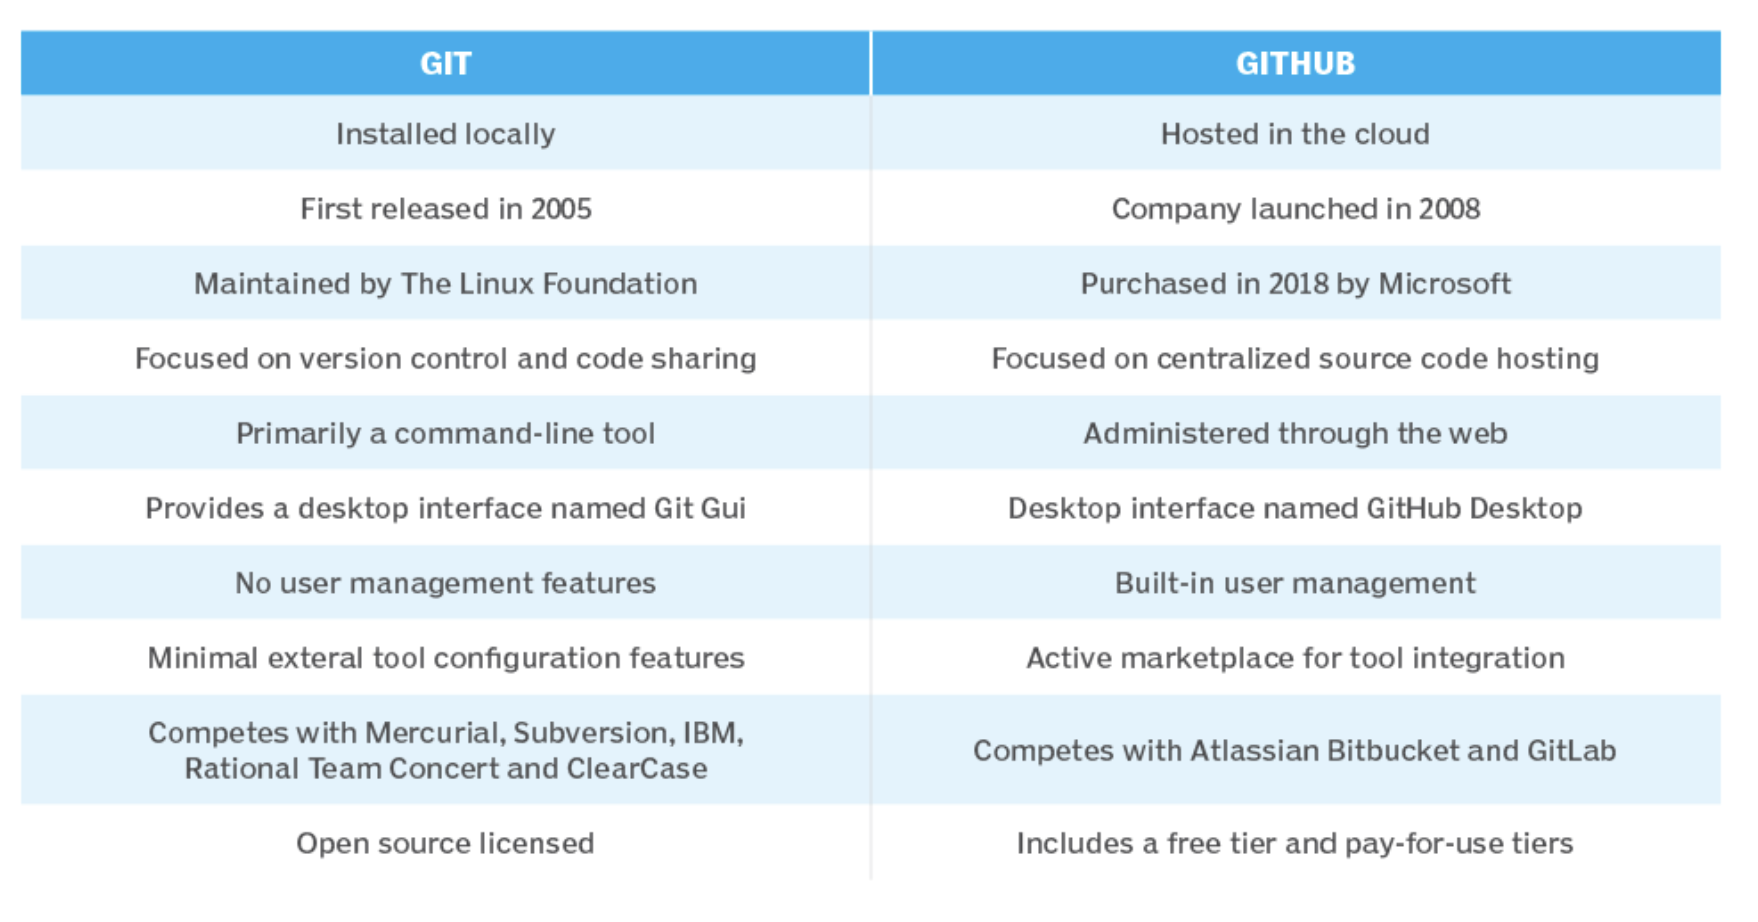
\includegraphics[scale=0.4]{2}} 

}


\frame{
\frametitle{How to Use Git}

%Install: git --version (osx)\\
%https://git-scm.com/book/en/v2/Getting-Started-Installing-Git

\centerline{
\includegraphics[scale=0.48]{9}}

}


\frame{
\frametitle{Setting up Git}

%Install: git --version (osx)\\
%https://git-scm.com/book/en/v2/Getting-Started-Installing-Git

\centerline{Install and Configure}

\begin{center}
\begin{itemize}
  \item git - -version
  \item git config - -global user.name "John Doe"
  \item git config - -global user.email johndoe@example.com
\end{itemize}
\end{center}

\vfill

\centerline{
\includegraphics[scale=0.16]{15}}

}

\frame{
\frametitle{Using Git}


\centerline{Initializing a Repository in an Existing Directory} 	

\begin{center}
\begin{itemize}
  \item git init
  \item git add myfavfile.txt
  \item git commit -m 'my first commit'
\end{itemize}
\end{center}


\centerline{You now have a Git repo with tracked files and an initial commit!}

\vfill

\centerline{
\includegraphics[scale=0.2]{16}}

}

\frame{
\frametitle{Using Git}

%Install: git --version (osx)\\
%https://git-scm.com/book/en/v2/Getting-Started-Installing-Git

\centerline{Cloning an Existing Repository}

\begin{center}
\begin{itemize}
  \item git clone https://github.com/mynewproject
\end{itemize}
\end{center}

\vfill

\centerline{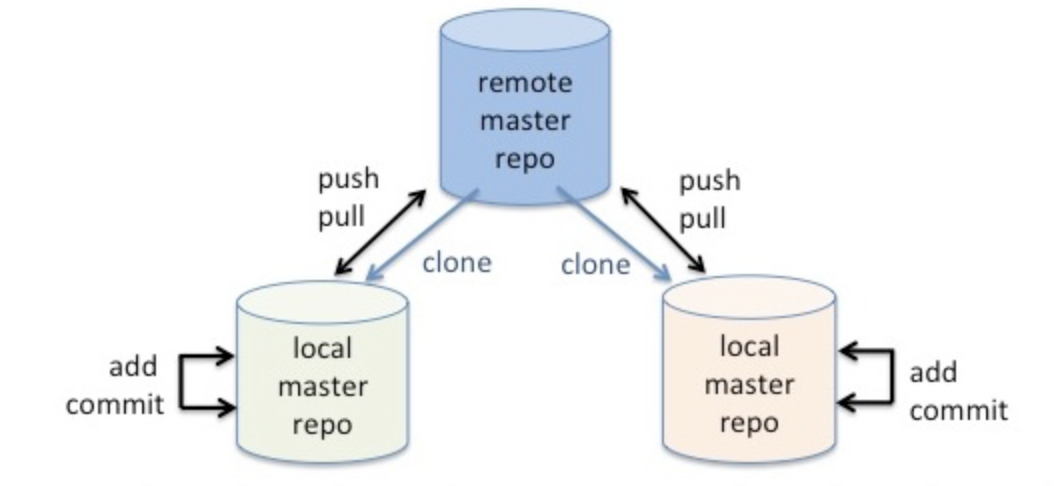
\includegraphics[scale=0.48]{14}}


}


\frame{
\frametitle{The General Workflow}

\centerline{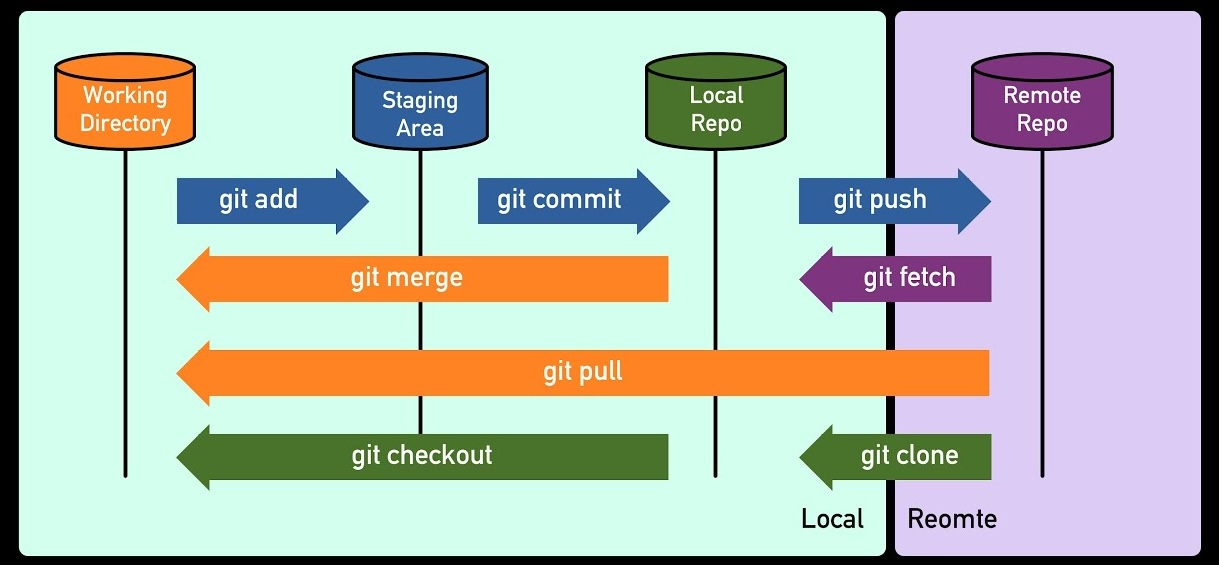
\includegraphics[scale=0.28]{10}}

}

\frame{
\frametitle{The General Workflow}

\centerline{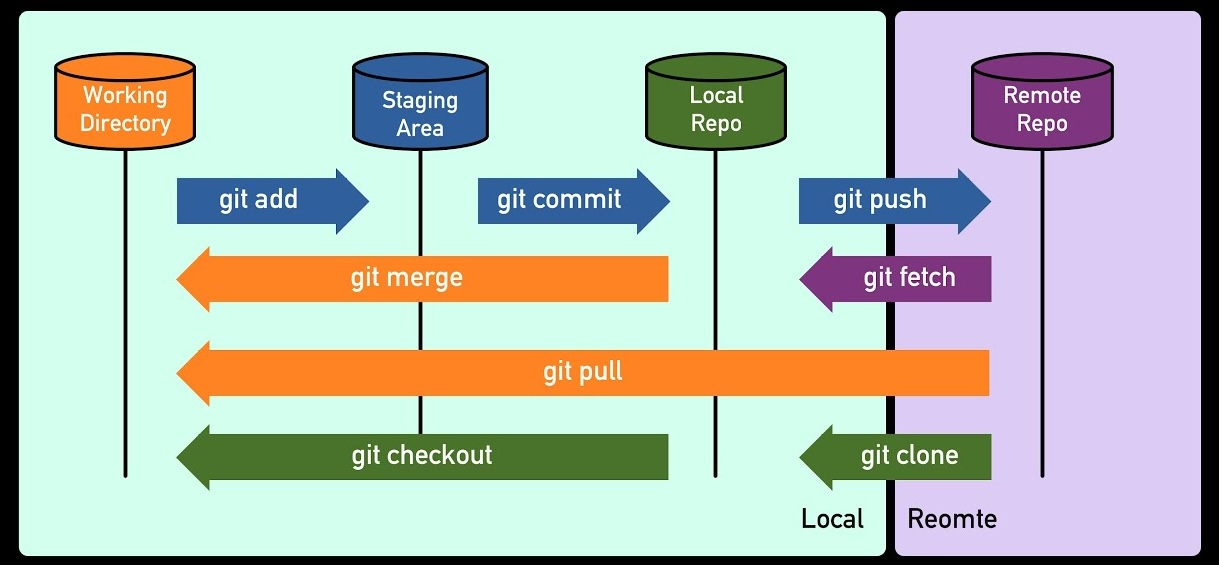
\includegraphics[scale=0.25]{10}}

\vfill

\centerline{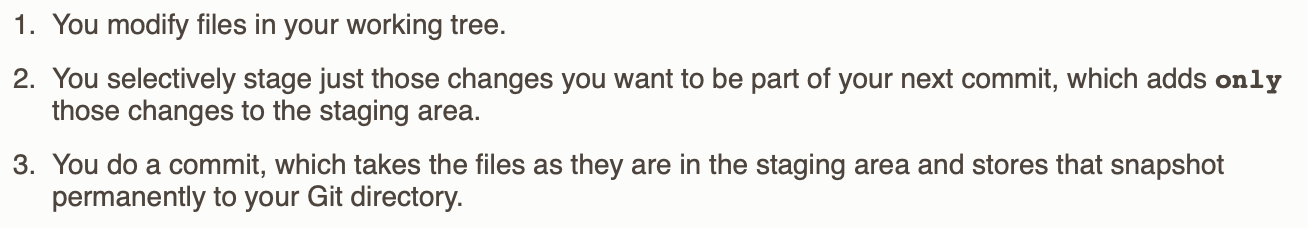
\includegraphics[scale=0.5]{13}}

}


\frame{
\frametitle{When diving into Git...}

\centerline{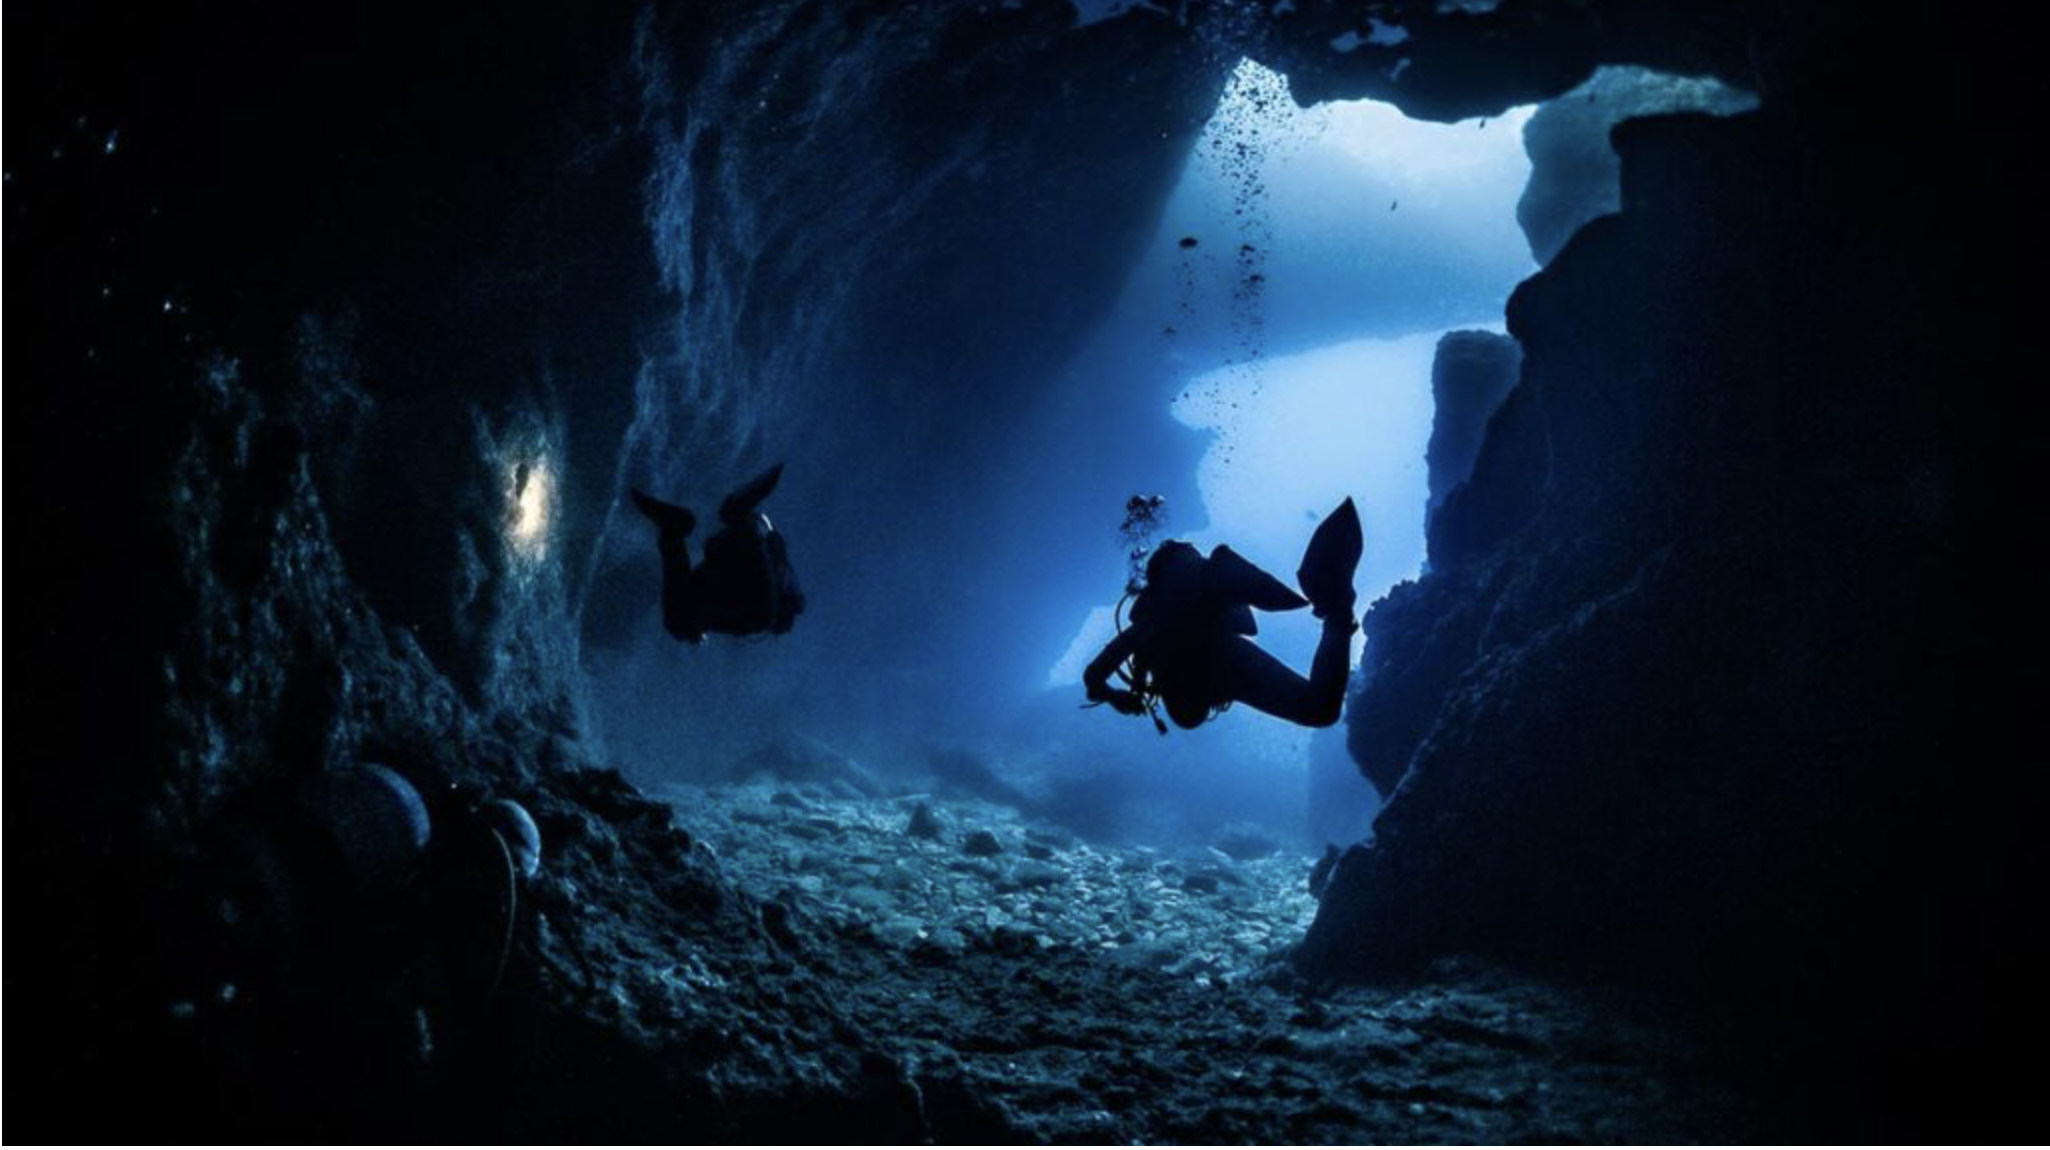
\includegraphics[scale=0.32]{5}} 

}

\frame{
\frametitle{Your path can be simple...}


\centerline{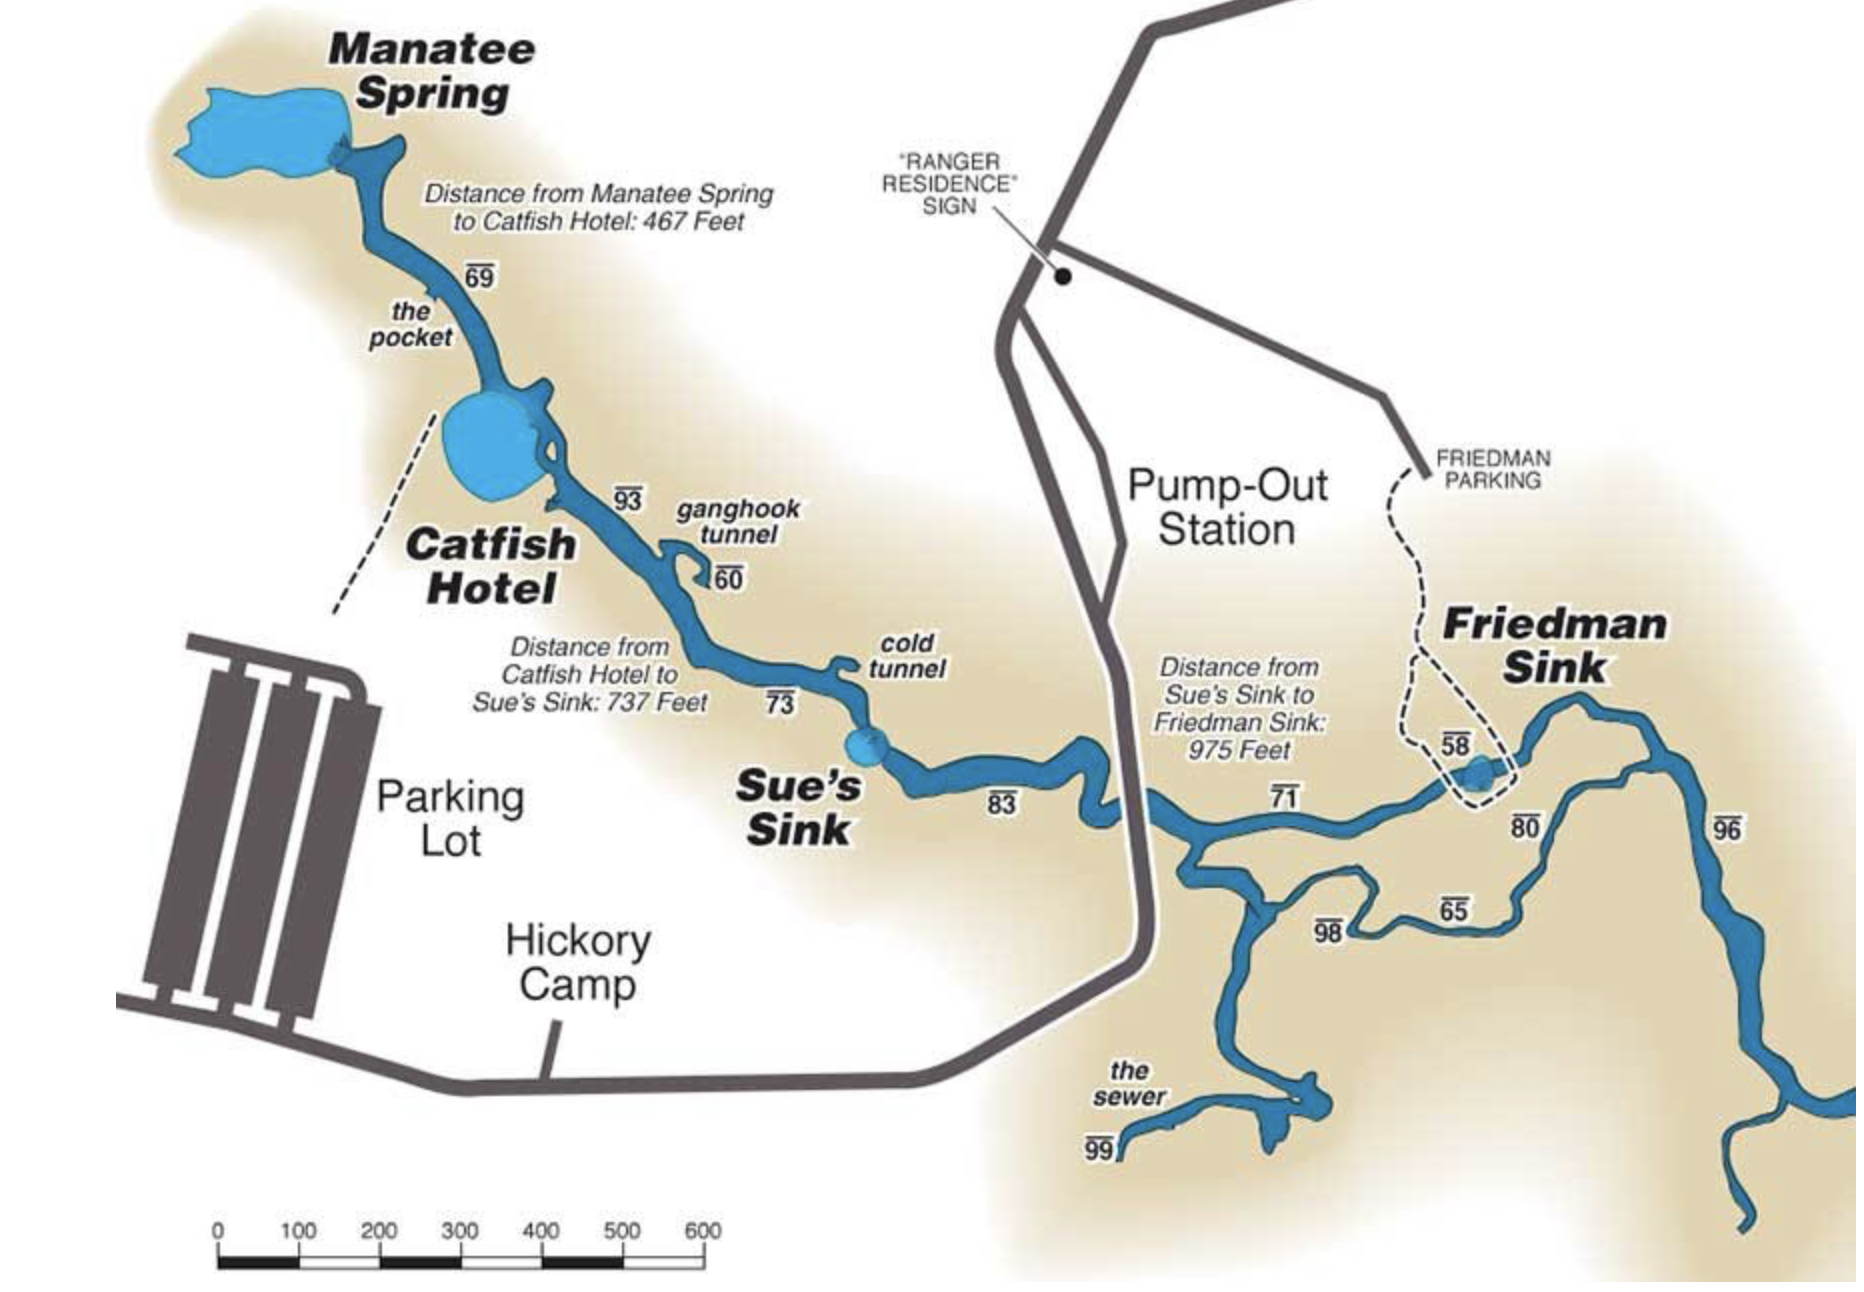
\includegraphics[scale=0.28]{6}} 

}

\frame{
\frametitle{Or as complicated as you like.}

\centerline{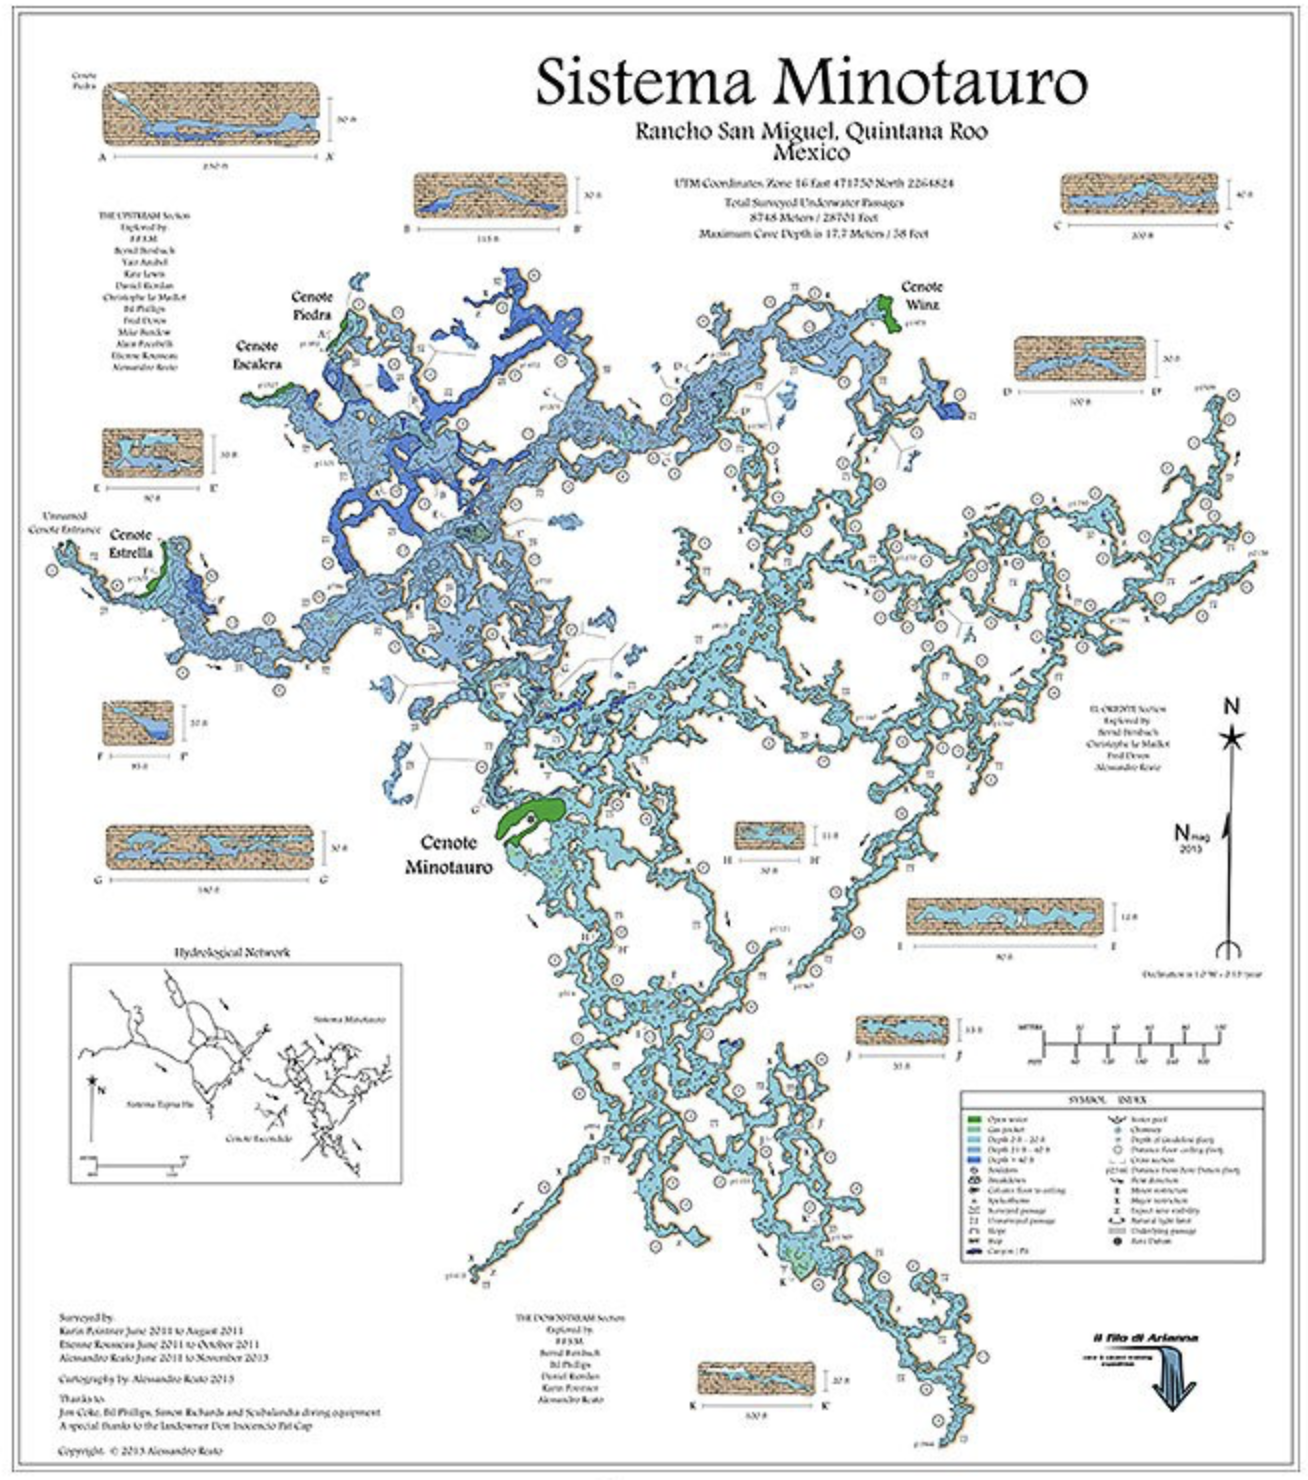
\includegraphics[scale=0.28]{7}} 

}

\frame{
\frametitle{Tools For Your Journey}

\centerline{GitHub, GitLab, and BitBucket for online servers}
\vfill

\centerline{Gitkraken for your Desktop}
\vfill

\centerline{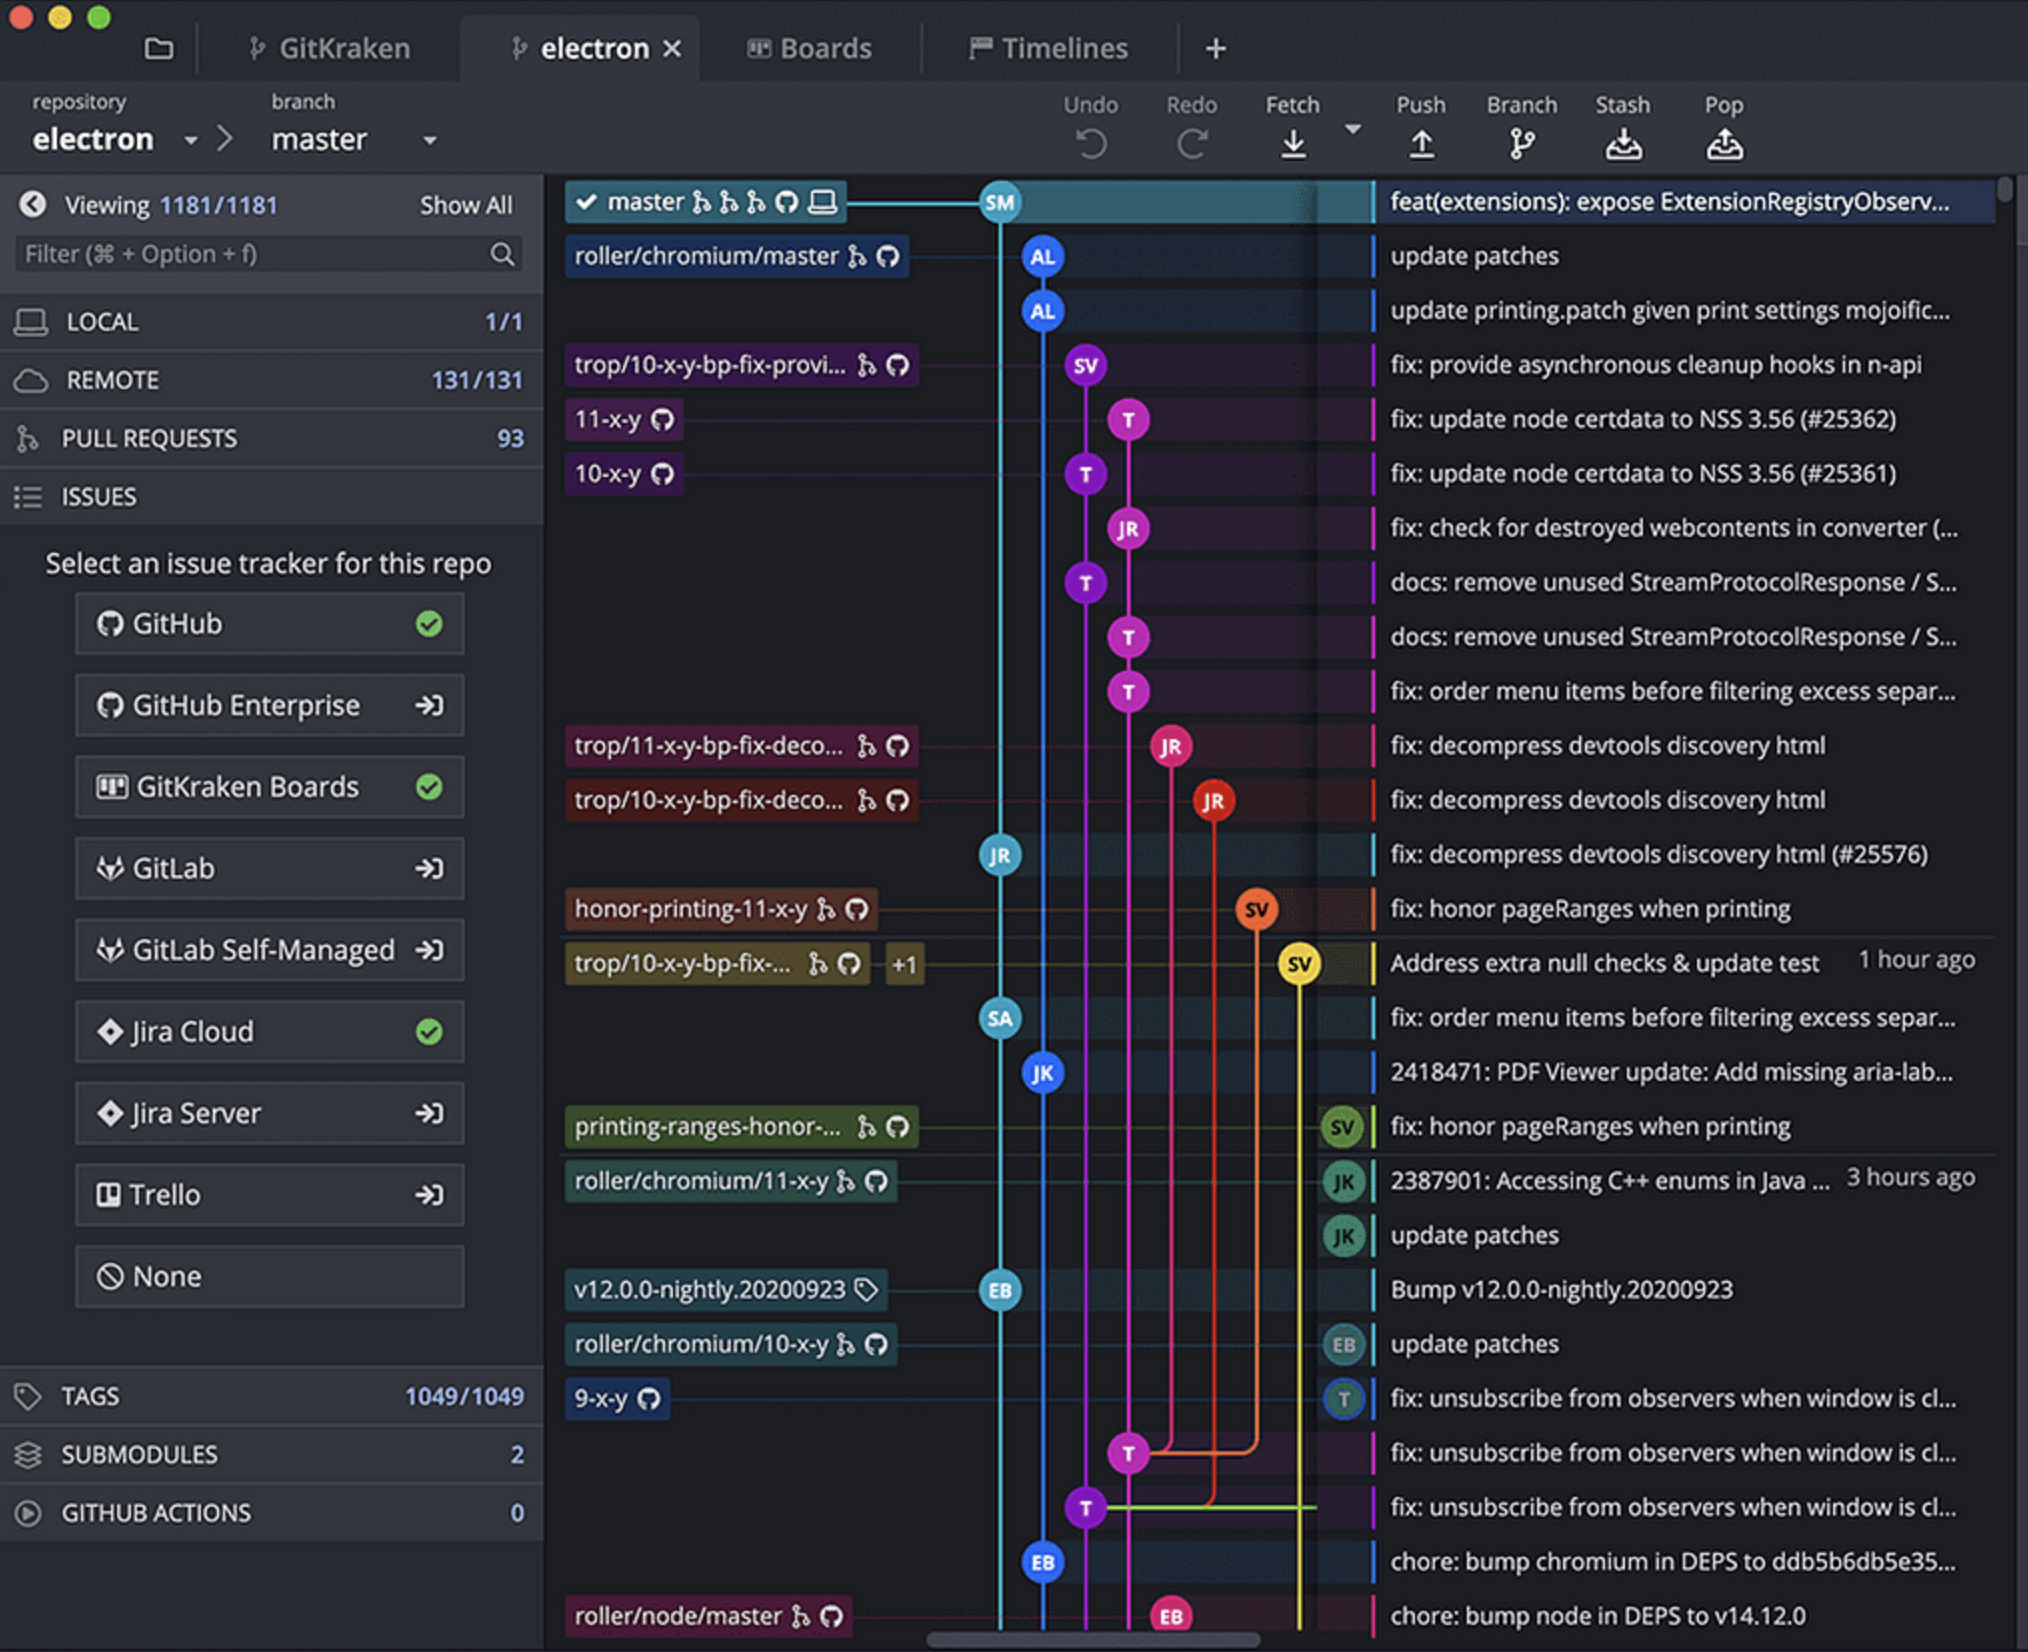
\includegraphics[scale=0.22]{18}} 

}




\section{\scshape LaTeX}
\subsection{LaTeX}


\frame{
\frametitle{History of Tex and LaTeX}

\begin{center}
1977 Donald Knuth developed Tex-- a computer language and program designed for use in typesetting; in particular, for typesetting math and other technical material.
\end{center}


\centerline{LaTeX was  written in the early 1980s by Leslie Lamport.}
\vfill

\begin{center}
TeX handles the document layout, while LaTeX handles\\ the content side for document processing.
\end{center}

\centerline{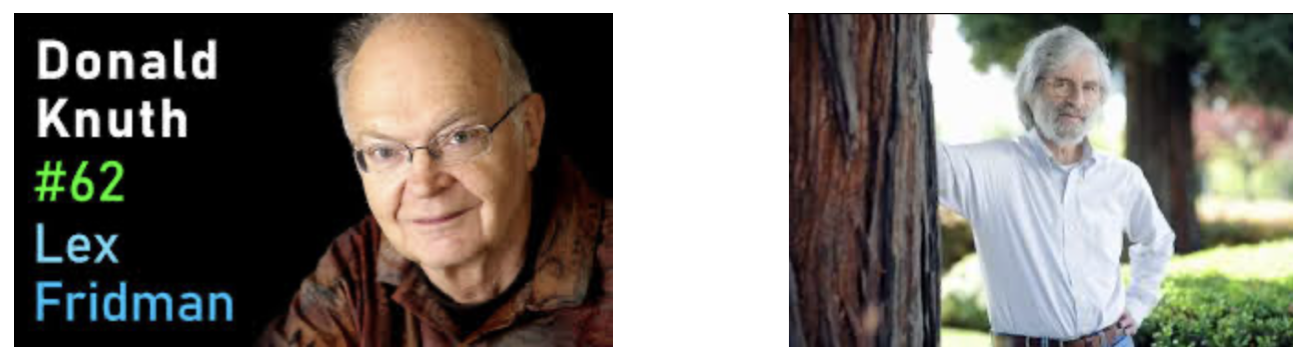
\includegraphics[scale=0.42]{21}} 

}

\frame{
\frametitle{Bonus Question 2!}

\centerline{What does TeX stand for?}

}


\frame{
\frametitle{Bonus Question 2!}

\centerline{What does TeX stand for?}



$$ \tau \epsilon \chi $$


}

\frame{
\frametitle{How to Use LaTeX}

\centerline{Installation}
\vfill

\centerline{https://www.latex-project.org}
\vfill

\centerline{
\includegraphics[scale=0.22]{19}} 

}

\frame{
\frametitle{Cool Stuff in LaTeX}

\centerline{Graphics with the Tikz package}
\vfill


\centerline{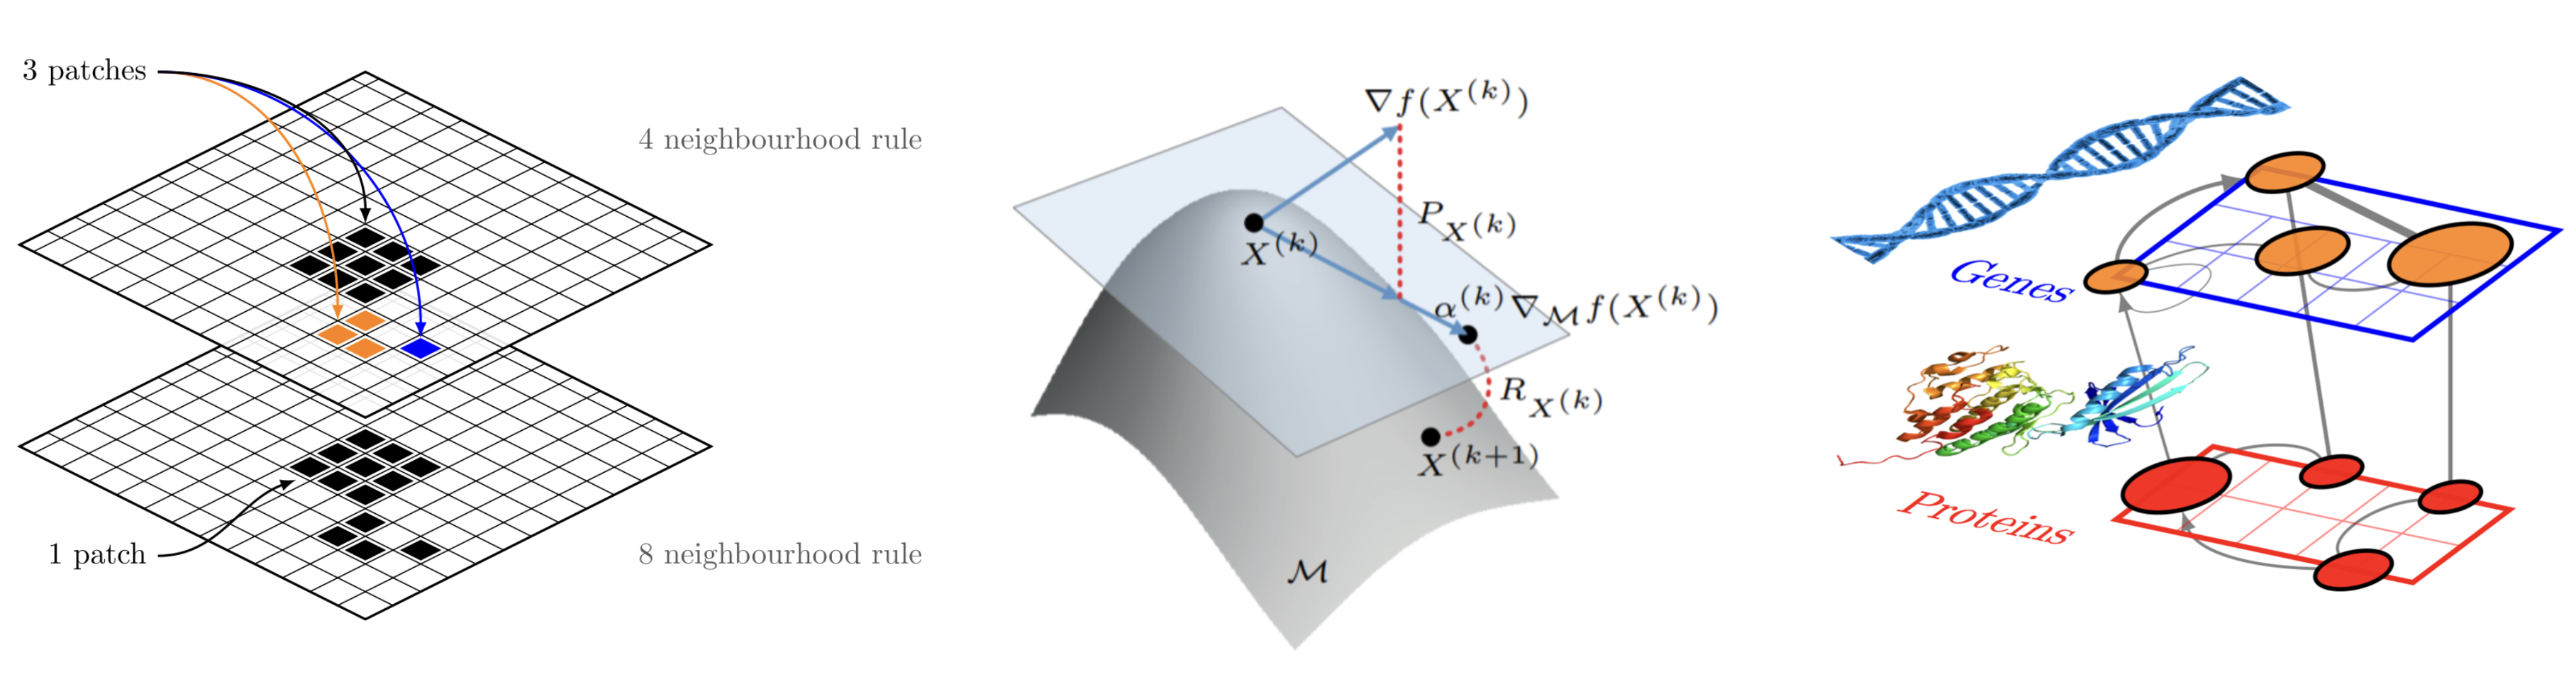
\includegraphics[scale=0.18]{20}} 

\vfill


\centerline{More than just Typesetting!}

}

\section{\scshape Surprise!}
\subsection{Surprise!}

\frame{
\frametitle{This Entire Presentation Was Done\\ in Git and \LaTeX !}

}

\section{\scshape Summary}
\subsection{Summary}

\frame{
\frametitle{Summary}

}

\frame{
\frametitle{Resources}

https://git-scm.com/book/en/v2

}

\end{document}


